\PassOptionsToPackage{unicode=true}{hyperref} % options for packages loaded elsewhere
\PassOptionsToPackage{hyphens}{url}
%
\documentclass[]{book}
\usepackage{lmodern}
\usepackage{amssymb,amsmath}
\usepackage{ifxetex,ifluatex}
\usepackage{fixltx2e} % provides \textsubscript
\ifnum 0\ifxetex 1\fi\ifluatex 1\fi=0 % if pdftex
  \usepackage[T1]{fontenc}
  \usepackage[utf8]{inputenc}
  \usepackage{textcomp} % provides euro and other symbols
\else % if luatex or xelatex
  \usepackage{unicode-math}
  \defaultfontfeatures{Ligatures=TeX,Scale=MatchLowercase}
\fi
% use upquote if available, for straight quotes in verbatim environments
\IfFileExists{upquote.sty}{\usepackage{upquote}}{}
% use microtype if available
\IfFileExists{microtype.sty}{%
\usepackage[]{microtype}
\UseMicrotypeSet[protrusion]{basicmath} % disable protrusion for tt fonts
}{}
\IfFileExists{parskip.sty}{%
\usepackage{parskip}
}{% else
\setlength{\parindent}{0pt}
\setlength{\parskip}{6pt plus 2pt minus 1pt}
}
\usepackage{hyperref}
\hypersetup{
            pdftitle={Mini-Workshop Panel Data Analysis},
            pdfauthor={Marko Bachl (mit Material von Michael Scharkow)},
            pdfborder={0 0 0},
            breaklinks=true}
\urlstyle{same}  % don't use monospace font for urls
\usepackage{color}
\usepackage{fancyvrb}
\newcommand{\VerbBar}{|}
\newcommand{\VERB}{\Verb[commandchars=\\\{\}]}
\DefineVerbatimEnvironment{Highlighting}{Verbatim}{commandchars=\\\{\}}
% Add ',fontsize=\small' for more characters per line
\usepackage{framed}
\definecolor{shadecolor}{RGB}{248,248,248}
\newenvironment{Shaded}{\begin{snugshade}}{\end{snugshade}}
\newcommand{\AlertTok}[1]{\textcolor[rgb]{0.94,0.16,0.16}{#1}}
\newcommand{\AnnotationTok}[1]{\textcolor[rgb]{0.56,0.35,0.01}{\textbf{\textit{#1}}}}
\newcommand{\AttributeTok}[1]{\textcolor[rgb]{0.77,0.63,0.00}{#1}}
\newcommand{\BaseNTok}[1]{\textcolor[rgb]{0.00,0.00,0.81}{#1}}
\newcommand{\BuiltInTok}[1]{#1}
\newcommand{\CharTok}[1]{\textcolor[rgb]{0.31,0.60,0.02}{#1}}
\newcommand{\CommentTok}[1]{\textcolor[rgb]{0.56,0.35,0.01}{\textit{#1}}}
\newcommand{\CommentVarTok}[1]{\textcolor[rgb]{0.56,0.35,0.01}{\textbf{\textit{#1}}}}
\newcommand{\ConstantTok}[1]{\textcolor[rgb]{0.00,0.00,0.00}{#1}}
\newcommand{\ControlFlowTok}[1]{\textcolor[rgb]{0.13,0.29,0.53}{\textbf{#1}}}
\newcommand{\DataTypeTok}[1]{\textcolor[rgb]{0.13,0.29,0.53}{#1}}
\newcommand{\DecValTok}[1]{\textcolor[rgb]{0.00,0.00,0.81}{#1}}
\newcommand{\DocumentationTok}[1]{\textcolor[rgb]{0.56,0.35,0.01}{\textbf{\textit{#1}}}}
\newcommand{\ErrorTok}[1]{\textcolor[rgb]{0.64,0.00,0.00}{\textbf{#1}}}
\newcommand{\ExtensionTok}[1]{#1}
\newcommand{\FloatTok}[1]{\textcolor[rgb]{0.00,0.00,0.81}{#1}}
\newcommand{\FunctionTok}[1]{\textcolor[rgb]{0.00,0.00,0.00}{#1}}
\newcommand{\ImportTok}[1]{#1}
\newcommand{\InformationTok}[1]{\textcolor[rgb]{0.56,0.35,0.01}{\textbf{\textit{#1}}}}
\newcommand{\KeywordTok}[1]{\textcolor[rgb]{0.13,0.29,0.53}{\textbf{#1}}}
\newcommand{\NormalTok}[1]{#1}
\newcommand{\OperatorTok}[1]{\textcolor[rgb]{0.81,0.36,0.00}{\textbf{#1}}}
\newcommand{\OtherTok}[1]{\textcolor[rgb]{0.56,0.35,0.01}{#1}}
\newcommand{\PreprocessorTok}[1]{\textcolor[rgb]{0.56,0.35,0.01}{\textit{#1}}}
\newcommand{\RegionMarkerTok}[1]{#1}
\newcommand{\SpecialCharTok}[1]{\textcolor[rgb]{0.00,0.00,0.00}{#1}}
\newcommand{\SpecialStringTok}[1]{\textcolor[rgb]{0.31,0.60,0.02}{#1}}
\newcommand{\StringTok}[1]{\textcolor[rgb]{0.31,0.60,0.02}{#1}}
\newcommand{\VariableTok}[1]{\textcolor[rgb]{0.00,0.00,0.00}{#1}}
\newcommand{\VerbatimStringTok}[1]{\textcolor[rgb]{0.31,0.60,0.02}{#1}}
\newcommand{\WarningTok}[1]{\textcolor[rgb]{0.56,0.35,0.01}{\textbf{\textit{#1}}}}
\usepackage{longtable,booktabs}
% Fix footnotes in tables (requires footnote package)
\IfFileExists{footnote.sty}{\usepackage{footnote}\makesavenoteenv{longtable}}{}
\usepackage{graphicx,grffile}
\makeatletter
\def\maxwidth{\ifdim\Gin@nat@width>\linewidth\linewidth\else\Gin@nat@width\fi}
\def\maxheight{\ifdim\Gin@nat@height>\textheight\textheight\else\Gin@nat@height\fi}
\makeatother
% Scale images if necessary, so that they will not overflow the page
% margins by default, and it is still possible to overwrite the defaults
% using explicit options in \includegraphics[width, height, ...]{}
\setkeys{Gin}{width=\maxwidth,height=\maxheight,keepaspectratio}
\setlength{\emergencystretch}{3em}  % prevent overfull lines
\providecommand{\tightlist}{%
  \setlength{\itemsep}{0pt}\setlength{\parskip}{0pt}}
\setcounter{secnumdepth}{5}
% Redefines (sub)paragraphs to behave more like sections
\ifx\paragraph\undefined\else
\let\oldparagraph\paragraph
\renewcommand{\paragraph}[1]{\oldparagraph{#1}\mbox{}}
\fi
\ifx\subparagraph\undefined\else
\let\oldsubparagraph\subparagraph
\renewcommand{\subparagraph}[1]{\oldsubparagraph{#1}\mbox{}}
\fi

% set default figure placement to htbp
\makeatletter
\def\fps@figure{htbp}
\makeatother

\usepackage{booktabs}
\usepackage[]{natbib}
\bibliographystyle{apalike}

\title{Mini-Workshop Panel Data Analysis}
\author{Marko Bachl (mit Material von Michael Scharkow)}
\date{Sommersemester 2020 \textbar{} IJK Hannover}

\begin{document}
\maketitle

{
\setcounter{tocdepth}{1}
\tableofcontents
}
\hypertarget{uxfcberblick}{%
\chapter{Überblick}\label{uxfcberblick}}

\hypertarget{inhalt-des-virtuellen-mini-workshops}{%
\section{Inhalt des virtuellen Mini-Workshops}\label{inhalt-des-virtuellen-mini-workshops}}

\begin{itemize}
\item
  Der Mini-Workshop bietet eine \emph{pragmatische} Einführung in die Analyse von Panel-Daten aus Erhebungen mit mindestens drei Wellen. Konkret liegt der Fokus auf sogenannten \emph{micro panels}, also Datensätzen mit relativ vielen Fällen und relativ wenigen Messzeitpunkten (das klassische Befragungspanel).
\item
  In der Analyse beschränken uns hier auf Varianten der \emph{linearen} Regressionsmodelle. Wir beginnen mit den grundlgenden \emph{fixed effects} und \emph{random effects} Modellen. Dann betrachten wir das \emph{within-between} Modell, das als eine Integration des \emph{fixed effects} Modell in das \emph{random effects} Modell verstanden werden kann. Dies ist auch eine gute Grundlage für den Einstieg in verschiedene Erweiterungen, zum Beispiel zu verallgemeinerten linearen Modellen oder zu Wachstumskurvenmodellen. Diese sind aber nicht Teil dieses Mini-Workshops.
\item
  Wir schätzen die Modelle mit etablierten \emph{least-squares} und \emph{maximum likelihood} Methoden. Gerade bei den \emph{within-between} Modellen sind bayesianische Schätzmethoden, z.B. \emph{MCMC sampling} (implementiert in \href{https://mc-stan.org/}{Stan}), unabhängig von den statistisch-philosophischen, sehr interessant. Bei Interesse kann ich nur empfehlen, hier einen Einstieg zu finden.
\item
  Zur Aufbereitung der Daten, Visualisierung und Modell-Schätzung verwenden wir \texttt{R} mit dem \texttt{tidyverse} und eine kleine Zahl speziallisierter Pakete für die Modellschätzung. Der Fokus des Workshops liegt aber auf der substantiellen Arbeit mit den Modellen, nicht auf der Umsetzung in \texttt{R}.
\end{itemize}

\hypertarget{welche-inhalte-wir-nicht-behandeln}{%
\section{Welche Inhalte wir nicht behandeln}\label{welche-inhalte-wir-nicht-behandeln}}

\begin{itemize}
\item
  Der Workshop ist kein Statistik- oder Ökonometrie-Kurs. Ich bin --- wie auch ihr --- ausgebildeter Sozialwissenschaftler. Die statistischen Grundlagen, auf denen der Workshop aufbaut, gehen aus den Grundlagentexten \citep{bellExplainingFixedEffects2015, vaiseyWhatYouCan2017} hervor.
\item
  Grundkentnisse in \texttt{R} setze ich voraus, insbesondere Datentransformationen innerhalb des \texttt{tidyverse}. Wir werden aber keine komplizierten Dinge in \texttt{R} tun. Auch ohne weiterführende \texttt{R}-Kenntnisse sollten die Inhalte des Workshops in Bezug auf die datenanalystischen Verfahren klar werden.
\item
  Wir werden nicht viel Zeit auf die verschiedenen Schätzer, deren Effizienz und Bias, die verschiedenen Algorithmen und Datentransformationen verwenden.
\item
  Wir werden keine Beweise oder Ableitungen besprechen. Wir setzen keine Kenntnisse in Matrixalgebra voraus --- weder meiner- noch eurerseits.
\item
  Wir behandeln einen sehr kleinen Ausschnitt möglicher Modelle für Panel-Daten. Der konzentrieren uns auf regressionsbasierte Modelle zur Schätzung kausaler Effekte. Damit behandeln wir insbesondere nicht die vielfälltigen Verfahren, die in einem SEM-Framework verortet sind: längsschnittliche Messmodelle, Prozessmodelle, (random intercept) cross-lagged panel Modelle, Latent State-Trait Modelle, etc.
\item
  Fehlende Daten (Panelmortalität, Ausfall von Einheiten in einzelnen Wellen) sind ein großes Thema in der Längsschnittanalyse. Wir werden es hier ignorieren, bis auf den Hinweis, dass alle Fälle, die in mindestens zwei bzw. drei Wellen Daten haben, grundsätzlich Informationen zur Schätzung beitragen.
\end{itemize}

\hypertarget{aufbau-des-workshops}{%
\section{Aufbau des Workshops}\label{aufbau-des-workshops}}

\begin{itemize}
\tightlist
\item
  Inhaltlicher Aufbau: Siehe Kapitel-Gliederung
\end{itemize}

\hypertarget{material}{%
\subsection*{Material}\label{material}}
\addcontentsline{toc}{subsection}{Material}

\begin{itemize}
\item
  Dieses Dokument + R Skripte: (Hoffentlich) mehr oder weniger selbsterklärendes Material

  \begin{itemize}
  \tightlist
  \item
    Kuratierte Form ist dieses HTML-Dokument
  \item
    Es gibt auch ein PDF, das ich aber nicht formatiert habe
  \end{itemize}
\item
  Screencast: Ich gehe über das Material und erkläre es auf der Audio-Spur. Mal sehen, wie hilfreich das ist. Die Screencasts stelle ich über das LMS zur Verfügung.
\item
  Übungen: Zu einigen Analysen gibt es Übungsaufgaben.

  \begin{itemize}
  \tightlist
  \item
    Bei der \emph{Wiederholung} geht es darum, die Modelle leicht zu verändern (durch Anpassen der \texttt{R}-Skripte aus dem Material) und die Ergebnisse der angepassten Modelle zu interpretieren.
  \item
    Bei der \emph{Anwendung} geht es darum, in Anlehung an die Beispiele eigene Modelle zu spezifizieren und diese zu interpretieren.
  \end{itemize}
\end{itemize}

\hypertarget{pakete}{%
\subsection*{Pakete}\label{pakete}}
\addcontentsline{toc}{subsection}{Pakete}

Wir verwenden die folgenden Pakete

\begin{Shaded}
\begin{Highlighting}[]
\ControlFlowTok{if}\NormalTok{ (}\OperatorTok{!}\KeywordTok{require}\NormalTok{(}\StringTok{"pacman"}\NormalTok{)) }\KeywordTok{install.packages}\NormalTok{(}\StringTok{"pacman"}\NormalTok{)}
\NormalTok{pacman}\OperatorTok{::}\KeywordTok{p_load}\NormalTok{(tidyverse)}
\KeywordTok{theme_set}\NormalTok{(}\KeywordTok{theme_bw}\NormalTok{())  }\CommentTok{# ggplot theme}

\KeywordTok{tibble}\NormalTok{(}\DataTypeTok{package =} \KeywordTok{c}\NormalTok{(}\StringTok{"R"}\NormalTok{, }\KeywordTok{sort}\NormalTok{(pacman}\OperatorTok{::}\KeywordTok{p_loaded}\NormalTok{()))) }\OperatorTok\StringTok{ }\KeywordTok{mutate}\NormalTok{(}\DataTypeTok{version =} \KeywordTok{map_chr}\NormalTok{(package, }
    \OperatorTok{~}\KeywordTok{as.character}\NormalTok{(pacman}\OperatorTok{::}\KeywordTok{p_version}\NormalTok{(}\DataTypeTok{package =}\NormalTok{ .x)))) }\OperatorTok\StringTok{ }\NormalTok{knitr}\OperatorTok{::}\KeywordTok{kable}\NormalTok{()}
\end{Highlighting}
\end{Shaded}

\begin{tabular}{l|l}
\hline
package & version\\
\hline
R & 3.6.2\\
\hline
dplyr & 0.8.4\\
\hline
forcats & 0.4.0\\
\hline
ggplot2 & 3.2.1\\
\hline
pacman & 0.5.1\\
\hline
purrr & 0.3.3\\
\hline
readr & 1.3.1\\
\hline
stringr & 1.4.0\\
\hline
tibble & 2.1.3\\
\hline
tidyr & 1.0.2\\
\hline
tidyverse & 1.3.0\\
\hline
\end{tabular}

\hypertarget{einfuxfchrung}{%
\chapter{Einführung}\label{einfuxfchrung}}

\hypertarget{luxe4ngsschnittdaten}{%
\section{Längsschnittdaten}\label{luxe4ngsschnittdaten}}

\hypertarget{begriffe}{%
\subsection*{Begriffe}\label{begriffe}}
\addcontentsline{toc}{subsection}{Begriffe}

\begin{itemize}
\tightlist
\item
  Wiederholte Querschnittserhebungen (time series cross sectional, TSCS): \(n\) unabhängige Fälle (repräsentativ für dieselbe Grundgesamtheit) zu mehreren Messzeitpunkten \(t\).
\item
  Zeitreihe: Eine Einheit mit vielen Messzeitpunkten (\(n = 1\), \(t > 30\)).
\item
  Paneldaten: Dieselben Einheiten mit wiederholten Messungen (\(n > 30\), \(t \ge 2\))

  \begin{itemize}
  \tightlist
  \item
    Macro panel: \(n\) klein, \(t\) groß (z.B. jährliche Untersuchung von Staaten, 1950--2015)
  \item
    Micro panel \(n\) groß, \(t\) klein (typisches Befragungspanel)
  \end{itemize}
\item
  In diesem Workshop geht es um \emph{micro panels} mit \(t > 2\)
\end{itemize}

\hypertarget{vorteile-von-paneldaten}{%
\subsection*{Vorteile von Paneldaten}\label{vorteile-von-paneldaten}}
\addcontentsline{toc}{subsection}{Vorteile von Paneldaten}

\begin{itemize}
\tightlist
\item
  Paneldaten erlauben die Identifikation von kausalen Effekten unter schwächeren Annahmen (im Vergleich zu Querschnittsdaten).

  \begin{itemize}
  \tightlist
  \item
    Wir haben einige (aber nicht perfekte!) Informationen über die zeitliche Abfolge von Veränderungen.
  \item
    Wir können untersuchen, ob, und wenn ja, wie ein Ereignis (eine Veränderung eines Prädiktors) das Kriterium verändert.
  \end{itemize}
\item
  Paneldaten erlauben die Untersuchung von individuellen Verläufen
\end{itemize}

\hypertarget{kausale-effekte-mit-paneldaten-schuxe4tzen}{%
\subsection*{Kausale Effekte mit Paneldaten schätzen}\label{kausale-effekte-mit-paneldaten-schuxe4tzen}}
\addcontentsline{toc}{subsection}{Kausale Effekte mit Paneldaten schätzen}

\hypertarget{bedingungen}{%
\subsubsection*{Bedingungen}\label{bedingungen}}
\addcontentsline{toc}{subsubsection}{Bedingungen}

\begin{enumerate}
\def\labelenumi{\arabic{enumi}.}
\tightlist
\item
  Kovariation zwischen \(X\) und \(Y\) (bivariate Korrelation \(r_{XY}\) )
\item
  \(X\) muss logischer vor \(Y\) liegen
\item
  Keine (nicht beobachteten) Störvariablen (kein \(Z\) mit kausalem Effekt auf \(X\) und \(Y\))
\end{enumerate}

\hypertarget{herausforderungen-auch-bzw.-gerade-mit-paneldaten}{%
\subsubsection*{Herausforderungen (auch bzw. gerade mit Paneldaten)}\label{herausforderungen-auch-bzw.-gerade-mit-paneldaten}}
\addcontentsline{toc}{subsubsection}{Herausforderungen (auch bzw. gerade mit Paneldaten)}

\begin{itemize}
\tightlist
\item
  Entsprechung der zeitlichen Entfalltung des Effekts und des Designs (Abstände, Verläufe)
\item
  Reliabilität und Konstruktstabilität

  \begin{itemize}
  \tightlist
  \item
    Reliabilität: Bei geringer Reliabilität beobachten wir Veränderungen, die aber auf Rauschen in der Messung zurückgehen.
  \item
    Reliabilität: Wenn die Messungen über die Zeit ihre Bedeutung verändern, modellieren wir keine Veränderung des latenten Konstrukts von Interesse.
  \end{itemize}
\item
  Panelmortalität und Paneleffekte

  \begin{itemize}
  \tightlist
  \item
    Panelmortalität: Einheiten (Befragte) fallen aus, möglicherweise systematisch mit Bezug auf die Konstrukte von Interesse
  \item
    Paneleffekte: Einheiten (Befragte) verändern sich durch die Messung (z.B. Lernen von Wissensfragen, Anregung durch Fragen zu Medienangeboten)
  \end{itemize}
\end{itemize}

\hypertarget{format-von-datensuxe4tzen-mit-paneldaten}{%
\subsection*{Format von Datensätzen mit Paneldaten}\label{format-von-datensuxe4tzen-mit-paneldaten}}
\addcontentsline{toc}{subsection}{Format von Datensätzen mit Paneldaten}

\begin{figure}
\centering
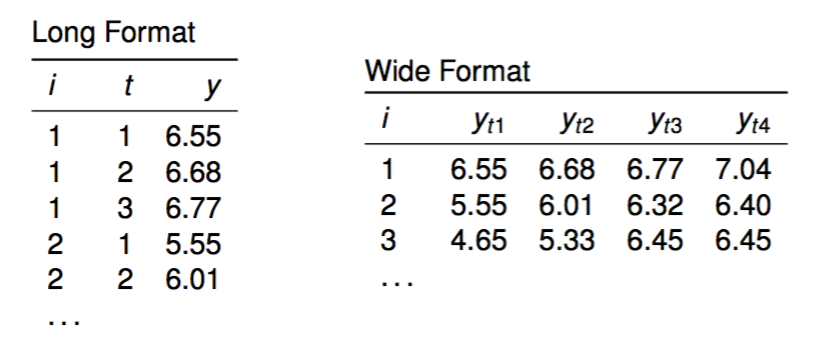
\includegraphics{figs/longwide.png}
\caption{\(i\) indiziert Einheiten, \(t\) indiziert Messzeitpunkte, \(y\) ist eine Variable}
\end{figure}

\begin{itemize}
\item
  Die Modelle in diesem Workshop nutzen das \emph{long format}
\item
  Datensätze können von einem ins andere Format transformiert werden, z.B. im \texttt{tidyverse}:

  \begin{itemize}
  \tightlist
  \item
    \texttt{tidyr::gather()} und \texttt{tidyr::spread()} oder
  \item
    \texttt{tidyr::pivot\_longer()} und \texttt{tidyr::pivot\_wider()}
  \end{itemize}
\end{itemize}

\hypertarget{beispiel-daten}{%
\section{Beispiel-Daten}\label{beispiel-daten}}

\begin{itemize}
\item
  sponsored by Jule Scheper und Sophie Bruns
\item
  KURZE INHALTLICHE BESCHREIBUNG

  \begin{itemize}
  \tightlist
  \item
    Ergebungszeitraum, Messzeitpunkte
  \item
    Repeated Measures
  \item
    Constant Measures
  \end{itemize}
\item
  Kurzer Auszug mit \texttt{summary} und \texttt{print}
\end{itemize}

\begin{Shaded}
\begin{Highlighting}[]
\NormalTok{d =}\StringTok{ }\KeywordTok{tibble}\NormalTok{(}\DataTypeTok{x =} \KeywordTok{rnorm}\NormalTok{(}\DecValTok{10}\NormalTok{), }\DataTypeTok{y =} \KeywordTok{rnorm}\NormalTok{(}\DecValTok{10}\NormalTok{))}
\end{Highlighting}
\end{Shaded}

\hypertarget{pooled-ols-wrong}{%
\section{Pooled OLS (WRONG!)}\label{pooled-ols-wrong}}

\begin{itemize}
\item
  Untersuchung des Effekts X -\textgreater{} Y
\item
  Einfachstes Modell: Regression X -\textgreater{} Y
\end{itemize}

\begin{Shaded}
\begin{Highlighting}[]
\KeywordTok{lm}\NormalTok{(y }\OperatorTok{~}\StringTok{ }\NormalTok{x, }\DataTypeTok{data =}\NormalTok{ d) }\OperatorTok\StringTok{ }\KeywordTok{summary}\NormalTok{(}\DataTypeTok{show.resid =}\NormalTok{ F)}
\end{Highlighting}
\end{Shaded}

\begin{verbatim}
## 
## Call:
## lm(formula = y ~ x, data = d)
## 
## Residuals:
##     Min      1Q  Median      3Q     Max 
## -2.2968 -0.8117 -0.2001  1.1529  1.8300 
## 
## Coefficients:
##             Estimate Std. Error t value Pr(>|t|)
## (Intercept)  0.49067    0.49586   0.990    0.351
## x            0.02564    0.45935   0.056    0.957
## 
## Residual standard error: 1.404 on 8 degrees of freedom
## Multiple R-squared:  0.0003894,  Adjusted R-squared:  -0.1246 
## F-statistic: 0.003116 on 1 and 8 DF,  p-value: 0.9569
\end{verbatim}

\hypertarget{warum-ist-pooled-ols-immer-falsch-statistische-theorie}{%
\subsection*{Warum ist Pooled OLS immer falsch? Statistische Theorie}\label{warum-ist-pooled-ols-immer-falsch-statistische-theorie}}
\addcontentsline{toc}{subsection}{Warum ist Pooled OLS immer falsch? Statistische Theorie}

\begin{enumerate}
\def\labelenumi{\arabic{enumi})}
\tightlist
\item
  Exogenitätsannahme ist verletzt, \(E(u_i|x_i) \neq 0\), da

  \begin{itemize}
  \tightlist
  \item
    Korrelationen zwischen den Variablen \(x\) gehen auf nicht gemessene Eigenschaften der Einheiten zurück, z.B. Eigenschaften der Person \(z_i\), die sowohl \(x_i\) als auch \(y_i\) beeinflussen.
  \item
    Auch bekannt als \emph{omitted variable bias}
  \item
    Könnte behoben werden, wenn alle \(z_i\) im Modell wären; diese Idee wird später wichtig
  \end{itemize}
\item
  Annahmen Homoskedastizität und unkorrelierte Residuen sind (wahrscheinlich) verletzt

  \begin{itemize}
  \tightlist
  \item
    Systematische Variaion der Residuen zwischen Einheiten
  \item
    Wahrscheinlich serielle Korreationen durch die zeitliche Abhängigkeit der Messungen
  \end{itemize}
\item
  Annahme der Unabhängigkeit der Bebobachtungen verletzt

  \begin{itemize}
  \tightlist
  \item
    Überschätzung der Information von abhängigen Fällen (dieselbe Information ist mehrmals im Datensatz)

    \begin{itemize}
    \tightlist
    \item
      Zu kleine Standardfehler, zu große Zahl der Freiheitsgrade in Signifikanz-Tests
    \end{itemize}
  \item
    Die wahre Fallzahl (effective sample size) ist kleiner als Zahl der Zeilen im Datensatz (\emph{long format})
  \end{itemize}
\end{enumerate}

\hypertarget{warum-ist-pooled-ols-immer-falsch-inhaltliche-uxfcberlegungen}{%
\subsection*{Warum ist pooled OLS immer falsch? Inhaltliche Überlegungen}\label{warum-ist-pooled-ols-immer-falsch-inhaltliche-uxfcberlegungen}}
\addcontentsline{toc}{subsection}{Warum ist pooled OLS immer falsch? Inhaltliche Überlegungen}

\begin{itemize}
\tightlist
\item
  Unser Ziel ist es, den wahren kausalen Effekt von \(X\) auf \(Y\) zu schätzen.
\item
  Pooled OLS vermischt aber zwei Quellen von Unterschieden in den Daten: Den (kausalen) Effekt innerhalb der Personen (within) und die Unterschiede zwischen Personen (between).
\item
  Within und between Effekte können sich in Größe und sogar in der Richtung unterscheiden!
\item
  Die Schätzung aus einem poold OLS Modell vermischt den kausalen Effekt und die interindividuellen Unterschiede.
\item
  In der Sprache von Interventionsstudien ist das ein Selbstselektions-Problem: Was passiert, wenn Personen, die vor dem Treatment \(x\) schon höhere Werte in \(y\) haben? \emph{X Evtl. anpassen an Datenbeispiel X}
\item
  Außerdem fällt auf, dass im einfachen OLS Modell nichts darauf hindeutet, dass es sich um Paneldaten handelt. Selbst wenn wir die genannten Probleme nicht hätten, hätten wir auch nichts durch die Paneldaten gewonnen.
\end{itemize}

\hypertarget{pooled-ols-within-und-between---eine-illustration}{%
\subsection*{Pooled OLS, within und between - eine Illustration}\label{pooled-ols-within-und-between---eine-illustration}}
\addcontentsline{toc}{subsection}{Pooled OLS, within und between - eine Illustration}

\begin{itemize}
\item
  Zum Abschluss noch ein imagninäres Beispiel, um den Unterschied von intraindividuellen (within) Effekten und interindividuellen Unterschieden zu verdeutlichen. Wir führen eine Panel-Studie mit acht Personen und sechs Messzeitpunkten zum Zusammenhang von Bier-Konsum und Hangover durch. Wir interessieren uns für die kausale Frage, ob mehr Bier zu einem schlimmeren Kater führt.
\item
  In der pooled OLS Analyse wird einfach die Rergressionsgerade durch alle Beobachung gelegt. Es zeigt sich ein negativer Zusammenhang. Je mehr Bier konsumiert wurde, desto schwächer fällt der Hangover aus.
\end{itemize}

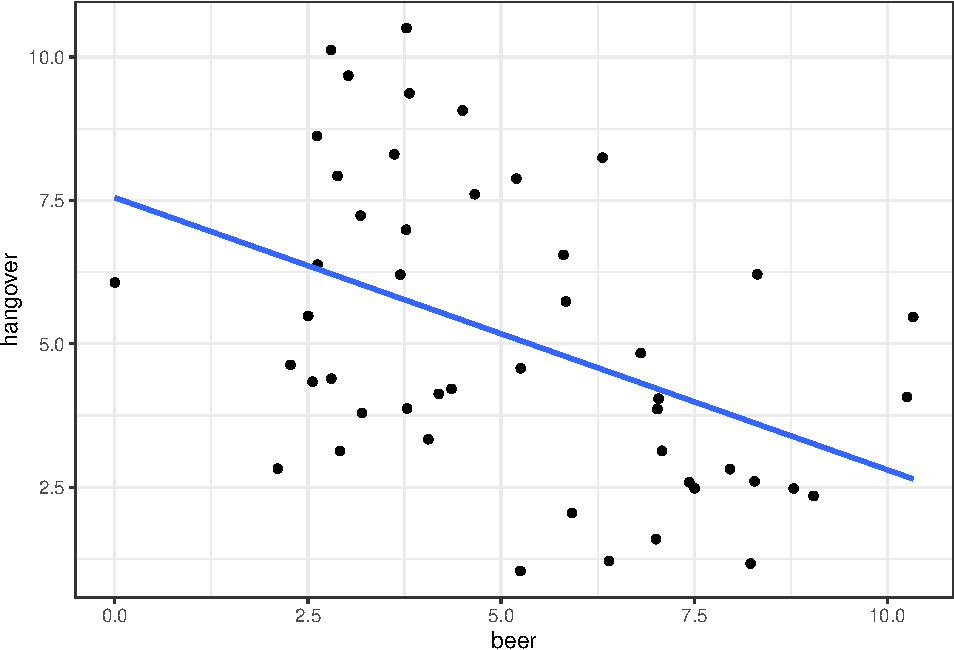
\includegraphics{workshop_panel_files/figure-latex/unnamed-chunk-7-1.pdf}

\begin{itemize}
\tightlist
\item
  Wenn wir aber für alle acht Personen separat den Zusammenhang zwischen Bierkonsum und Kater berechnen (so genanntes no pooling Modell), ergibt sich ein anderes Bild. Für alle Personen gilt mehr oder weniger deutlich: Je mehr Bier konsumiert wurde, desto stärker fällt der Hangover aus (within).
\end{itemize}

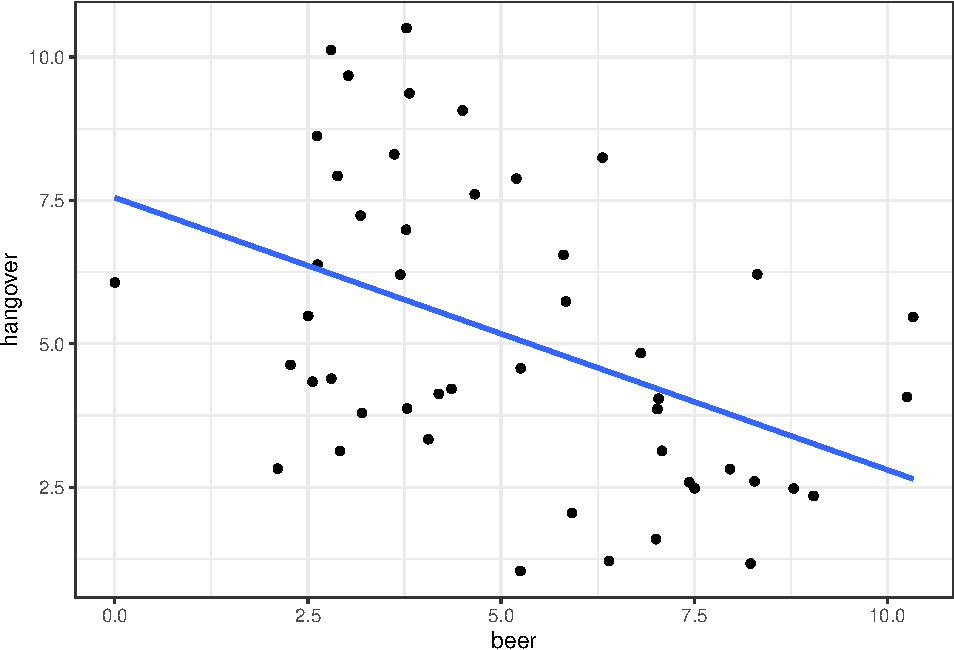
\includegraphics{workshop_panel_files/figure-latex/unnamed-chunk-8-1.pdf}

\begin{itemize}
\item
  Dazu kommt ein systematischer Unterschied zwischen den Personen (between): Personen, die im Durchschnitt mehr Bier trinken, haben im Durchschnitt einen schwächeren Hangover. Dies könnte eine nicht beobachte Drittvariable auf Ebene der Personen sein. Vielleicht trinken Personen, die wissen, dass sie nicht so anfällig für einen Hangover sind, mehr, während Personen, die immer einen starken Kater haben, schon aus Angst vor dem nächsten Tag weniger trinken. Oder es ist ein Gewöhnungseffekt: Personen, die häufig viel trinken, gewöhnen sich an den Kater und nehmen ihn als weniger schlimm wahr. Oder mit Lemmy: ``A kid once said to me ``Do you get hangovers?'' I said, ``To get hangovers you have to stop drinking.''
\item
  Mit den vorliegenden Daten können wir die Frage nach dem Prozess nicht beantworten, da wir die Drittvariable nicht gemessen haben. Wir können aber \emph{alle} Variablen kontrollieren, die auf Personenebene liegen, z.B., indem wir wie in der Abbildung für jede Person ein separates Modell schätzen. Dann können Unterschiede zwischen den Einheiten per Modelldefinition keinen Einfluss auf die Schätzung haben. Etwas ähnliches passiert im \emph{fixed effects} Modell, das wir im nächsten Abschnitt besprechen.
\end{itemize}

\hypertarget{fixed-effects-modelle}{%
\chapter{Fixed effects Modelle}\label{fixed-effects-modelle}}

\hypertarget{konzeptionelle-einfuxfchrung}{%
\section{Konzeptionelle Einführung}\label{konzeptionelle-einfuxfchrung}}

\begin{itemize}
\tightlist
\item
  Im ersten Teil des Abschnitts zu \emph{fixed effects} Modellen beschäftigen wir uns mit den Grundlagen der Modellierung. Dazu nutzen wir die bekannte Funktion \texttt{stats::lm()} (übliche OLS-Schätzung linearer Modelle in R).
\end{itemize}

\hypertarget{wie-kuxf6nnen-wir-den-kauselen-within-person-effekt-mit-paneldaten-schuxe4tzen}{%
\subsection*{Wie können wir den kauselen (within-person) Effekt mit Paneldaten schätzen?}\label{wie-kuxf6nnen-wir-den-kauselen-within-person-effekt-mit-paneldaten-schuxe4tzen}}
\addcontentsline{toc}{subsection}{Wie können wir den kauselen (within-person) Effekt mit Paneldaten schätzen?}

\begin{enumerate}
\def\labelenumi{\arabic{enumi})}
\tightlist
\item
  Separate OLS Modelle für jede Person schätzen und Koeffizeinten mitteln (no pooling).
\item
  Alle \(X\) und \(Y\) Variablen um die Mittelwerte der Person zentrieren (within transformation).
\item
  Dummy-Variablen für jede Person in das Regressionsmodell aufnehmen (least squares dummy variables {[}LSDV{]} estimation).
\end{enumerate}

\begin{itemize}
\tightlist
\item
  Alle drei Varianten entfernen die (beobachteten und nicht beobachten,) über die Zeit konstanten Unterschiede zwischen den Personen.
\item
  Varianten 2 und 3 entsprechen dem klassischen \emph{fixed effects} Modell. Die Unterschiede zwischen den Personen werden kontrolliert, indem die personenspezifischen Mittelwerte vor der Schätzung entfernt werden (2) oder für jede Person im Modell geschätzt werden (3).

  \begin{itemize}
  \tightlist
  \item
    \(y_{it} = \beta' x_{it}' + \alpha_i + u_{it}\) or \(y_{it}-\bar{y_{i}} = (x_{it} - \bar{x_{i}})'\beta + (u_{it} - \bar{u_{i}})\)
  \end{itemize}
\item
  In Variante 1 dürfen die kausalen within-person Effekte zwischen den Personen variieren. Unter der Annahme homogener Treatment-Effekte (entspricht der typischen Annahme im randomisierten Between-Subject-Experiment) entspricht das Ergebnis asymptotisch den Varianten 2 und 3.

  \begin{itemize}
  \tightlist
  \item
    Der Schätzer ist aber weniger effizient, da zufällige Unterschiede in den Effekten zwischen den Personen aufgegriffen werden.
  \item
    Im letzten Teil des Abschnitts zum within-between-Modell kommen wir auf diesen Punkt zurück, wenn wir die Annahme homogener Treatment-Effekte lockern.
  \end{itemize}
\end{itemize}

\hypertarget{random-effects-models}{%
\chapter{Random effects models}\label{random-effects-models}}

XXX

\hypertarget{within-between-models}{%
\chapter{Within-between models}\label{within-between-models}}

XXX

\bibliography{book.bib,packages.bib,references.bib}

\end{document}
